\chapter{Fur: An Intelligent Fault Tolerance System}
\label{c:fur}

This chapter describes how subsystems in Fur collaborate to provide fault tolerance
for applications. Then we will move 
on to describing how WuKong Master takes this FBP and policy to convert into 
low-level intermediate representation ready to be deployed. Lastly, we 
describe how the sensor network detect, recognize, and recover from failures.

\section{WuKong Applications}

~\ref{application} illustrates a typical WuKong application with components
connecting to form a small network. What this figure shows is that applications
are made of components, and components are connected through properties.
Any pair of properties form links that binds components together. Connected
components interact with each other based on the direction of the connection.
The properties on the left of a component are inputs to this component, to the
right side are the outputs of an component. Thus one can infer that
a connection cannot connect to both inputs or outputs of any pair of components
as both of them have the same data flow.

\section{Redundancy}

A typical fault tolerant distributed system is based on the concept of
redundancy and distributed systems usually have advantages to have spare
resources.

Spare resources addresses the first fundanmental characteristics of fault
tolerance that there is no single point of failure.

Redundancy in WuKong would be to duplicate the nodes that host critical
components with the intention to switch to one of the remaining
instances in case of a failure.

However, heterogeneous sensor network imposes a challenge to design a fault
tolerant system when compatible spare resources will have to be considered rather
than narrowing for identical spare resources for redundancy.

\section{Groups}
% Q: Why groups? What's the benefits for this abstraction in WuKong with profile
% framework? And how does it fit in?

I propose to use group abstraction to implement redundancy in WuKong
application.

Any component in the application can thought of a collection of nodes that might be
hosting this component. When the mapper in WuKong tries to find a mapping for
a component, instead of looking for just one node, it will try to find a number
of spare nodes to be part of the redundancy.

When a component needs to increase reliability, a group size is
specified for that component in the FBP as shown in~\ref{group_size}.

Every component can set a number greater than one to indicate the intended size
of the group of nodes which will be mapped to host this component. The
component will be called a \textit{component group}. The size of the group is
an positive integer that cannot be less than 1.

\subsection{Mapping for component groups}

As illustrated in~\ref{mapping}, a mapping consists of a set of application
components as shown as circles on the top of the figure, and a set of nodes
with a list of capability that certain application components could map to.

An application component can only map to compatible nodes. Compatible nodes are
nodes with features that match the desire features from the component
profile. For example, a temperature sensor component requires temperature
sensor feature. A node with a temperature sensor installed will have this
feature and it will be a compatible node for this component.

A software application component can be mapped to any node that is capable of
computation, but a hardware application component can only map to the nodes
that has the features corresponded to the component profile.

A valid mapping is a mapping would have all components mapped to at least one
compatible node or to the number of compatible nodes specified in group size,
that's the desire output for the mapper.

\subsubsection{Final algorithm}

For the mapper to find a valid mapping, we have to modify the algorithm to
consider multiple compatible nodes in questions at the same time. The~\ref{mapper} shown is used.

\begin{algorithm}
\caption{Generate Mapping with groups}
\label{mapper}
\begin{algorithmic}
\item test
\end{algorithmic}
\end{algorithm}

\begin{comment}
\section{Questions}

Q: Inclusion problem, how to solve it? How severe it is?

Q: How do mapper decide the relative locations between group members? How would
the system prevent lone nodes problem, where one node could be far far away
from the rest of the group, the cost of monitoring that node is so much that it
loses the effectiveness of heartbeats and producing so much messages that it
might saturated the network plus the hops between the nodes makes determining
the status of the node far less straightforward?

A: This is a legitimate concern, however we could assume that any node far far
away from the geographical location of other group members will not be
considered. WuKong Master mapper tries as hard as it can to find group members
that are close to each other by using location topological tree created by the
installers to prevent this from happening.

Q: Should we use anchor nodes to reduce hops between heartbeat messages? Should
we allow specialized nodes to monitor a subset of group memers?

A: Anchor nodes might sound attractive at first, but in reality, the more nodes
put in monitoring, the more bandwidth it would have to become, since those
anchor nodes is also at the risk of being dead, the leader of a group would
just be shifting its focus from monitoring the real member to this specialized
anchor node. This approach does not reduce the amount of traffic produce for
monitoring.

Q: How does the system recover from two consequtive failures in the network?


A: We assume a much simpler failure model where there can be at most one
failure happen at any point in time. It is a reasonable assumption given that
our system recover from failures fairly quickly (~2 secs) ....


Q: How does an application is being compiled into low level bytecode? And when
and how does WuKong reconfigure the nodes?


Q: What happen when an application is deployed? What is specifially at work?
\end{comment}


\section{Goal}


\section{Group abstraction}


\section{Policy}

\subsection{Fault tolerance category}


\section{Mapping}

\subsection{Matching}

\subsection{Translation}

\subsection{Compilation}

\subsection{Reprogramming}

\subsection{Reconfiguration}

\subsubsection{Member ranking}

% transition to failure diagnosis, and failure recovery, and member ranking
If application could specify a full ranking among a group, 
Whenever a leader died, a member has to replace its position.
Leader identification, successor of current leader.

 agent should specify whether this group has any ranking rules for a members. Whether there is a full ranking for current members and future members. This could lead to different actions reacting to similar events. ...



\section{Agent architecture}

This section will first go into details of how applications in a form of an
abstract graph are being managed in a distributed system after being compiled 
and transformed into lower bytecode representation, then I will further discuss 
how the agent architecture on every node collaborate to form groups that will 
be the basic unit of redundancy in the application to detect sensor failures, 
diagnosis the failure, and finally recover from failure.

~\ref{} illustrates the proposed agent architecture in the sensor network.
Every component in the application is converted into groups, which consists one
or more nodes, and one of them is a leader. Every group has only one leader.
Heartbeats are sent out from the members and leaders to monitor each other.

\subsection{Autonomous Systems}

Sensor networks composed of a large number of diverse subsystems. Subsystems
intertwined with complex relationships that prohibit human intervention.
Subsystems such as deployment, operation, reconfiguration, maintenance must be
automated.

The inability, passiveness to errors makes the past systems unable to deal with
perturbations, or unpredictable changes in the environment. Such systems know
a limited amount of patterns and trigger predefined actions when they encounter
these patterns. In order to make system adapt to new environment in a way
similar to biological systems, they need to react to events as a whole in
real-time.

\subsection{Distributed agents}

As our system consists of complex elements and subsystems mingled together, an
appropriate way to handle complex behaviors in decentralized systems is to
based it on a society of agents.~\cite{Minar1999}

\subsection{Towards failure detection}

As we mentioned earlier why sensor systems has to evolve to adapt to crutial,
ever changing environment, one of the first things a system could achieve that
goal is to detect failures autonomously.

\subsubsection{Group membership}

In our model, sensor networks consists of a diverse of sensor platforms, and some
subset of sensor nodes are equipped with similar sensors situated near each other.

Since sensor networks are inheritly concurrent, it is very hard to reason about
the states of the nodes in a distributed fashion. In order to provide fault
tolerance in the system, a number of nodes need to be in sync and form a group
to monitor and replace faulty node if necessary.

~\ref{} illustrates a running applications with three components: Temperature,
Light and Threshold. Every component is implemented by a group of sensors
hosting the same object that represents the component.

Every node consists of two agents, namely membership and controller as
illustrated in the~\ref{}. When application is deployed, every node is populated with a link table full of links and a list of objects representing the components on the application that are being assigned to.

Membership agent is there to maintain and update the membership list by
also managing a watchlist and a reportlist to receive/send heartbeat from/to.

\paragraph{Heartbeat and node failure}

% what is a failure, why we assume fail-stop failures

A failure in distributed system could come from different sources. Some nodes
might fail because of software bugs; some nodes might fail because of poor
wireless link quality caused by interference. One of the biggest challenges in
distributed systems is to be able to detect the types of failures when it
occurs correctly. Pulled between efficiency and reliability, decisions to make
individual sensor nodes at the same time able to detect failures with knowledge
of others but also have to reduce the amount of resources is essential for
designing a effective distributed system.

% Brief introduction to Byzentine failures

There is another type of failures caused by a completely different reasons.
Byzentine failures are failures inspired by the Byzentine General's Problem
where components of a system fail in arbitrary ways (besides stopping or
crashing) by processing requests incorrectly, corrupting local states, or
producing incorrect or inconsistent outputs.

% Why we choose fail-stop failures

As we assume society of cooperative agents, every agent in the system will
strive to be helpful, and share a common goal. This is strengthen by the fact
that the agent goals' are bootstrapped from a common source which is the WuKong
Master. However, nodes could still fail. In order to be consistent, we model
failure by whether a node could send messages or not. This is called
a fail-stop failure model.

% What we choose

A fail-stop failure model is a model in which sensor nodes are suspected of
failure when they stop sending messages which could caused by multitude of
reasons such as network partition, or software bugs.

% what is a heartbeat

Heartbeats are messages sent by individual nodes periodically to indicate to
the monitoring nodes its health~\cite{}.

~\ref{} illustrates some nodes sending heartbeats that detects
a failure when a number of expected consecutive heartbeats have not been
received.

% what is a failure in our model

A node is considered dead when it has not been sending heartbeats for more 
than 2 rounds of timeout.

\paragraph{Group setup}

The WuKong Master has already assigned an ordered list of nodes for every component,
every node would be able to know who are in their group for any particular
component.

Wielded with this knowledge, membership agent will setup all heartbeat links
between the nodes if not already.

Since the setup is asynchronous without lockstep, all nodes are free to do
whatever they want while others are being programmed. We added a random backoff
after the nodes are programmed to prevent the problem of nodes reporting 
failure when they startup, because when the node finished setup, the nodes it
is watching might not be finished reprogramming, thus it will delay its
heartbeat and exceed the timeout causing the node to send false alarm.

As illustrated by~\ref{}, every node has a leader which is elected when the
group is formed.

\begin{figure}[h!]
\caption{Node states}
\centering
    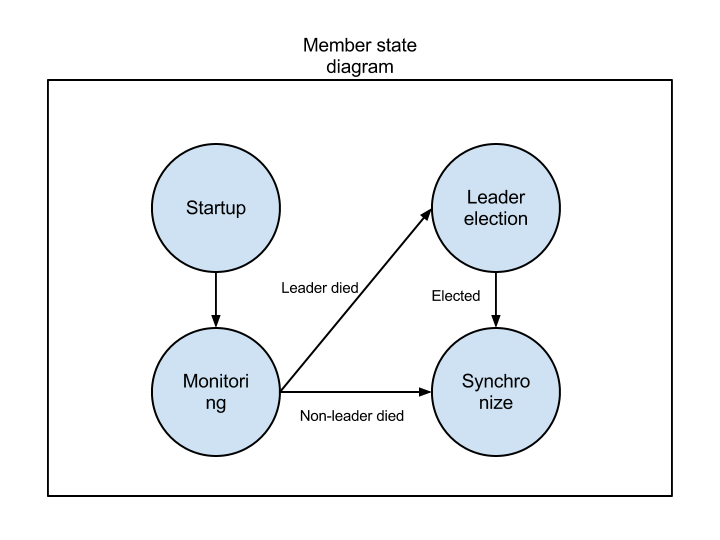
\includegraphics[width=\linewidth]{figures/node-states}
\end{figure}

\subsubsection{Connecting them up}

% what happened when a node fails?

When a node failed, or has not sent heartbeats for too long, a node failure
will be picked up by the monitoring nodes. However, a system is not fault
tolerant if it cannot decide who could be replacing the failing component. So
there must be some way to organize groups such that when a failure is detected,
a replacement could be decided.

% introduction to heartbeat network

It is possible that there will be multiple failures occurred in a timely
fashion. We need to be able to detect all possible failures within a group, so we need a heartbeat network.

% talk more about heartbeat network

Of course the structure of heartbeat communication pattern highly depends on the underlying network assumption and infrastructure of the application. To produce the most efficient network with the least connections, heartbeat network has to satisfy two properties.

\begin{enumerate}
\item Every node has to monitor at least one node other than itself
\item Every node can only has one node monitoring itself
\end{enumerate}

% why daisy chain, what's the benefits? How does it affect other fault
% tolerance policies?

A heartbeat network in the form of a daisy chain is one of the networks that
satisfy both properties as shown in~\ref{daisy_chain}. Every daisy chain heartbeat network monitors all nodes
in the group, given by the properties that every node has to monitor at least
one node and every node can only have one node monitor itself. So if there is
n nodes, there can be at most n nodes being monitored, every monitoring node
can only monitor one node, every node can only monitor node that others have
not, thus every node is monitored by only one unique node. Thus this daisy
chain guarantees every failure can be detected.

\begin{figure}[h!]
\label{daisy_chain}
\caption{Daisy Chain of heartbeats}
\centering
    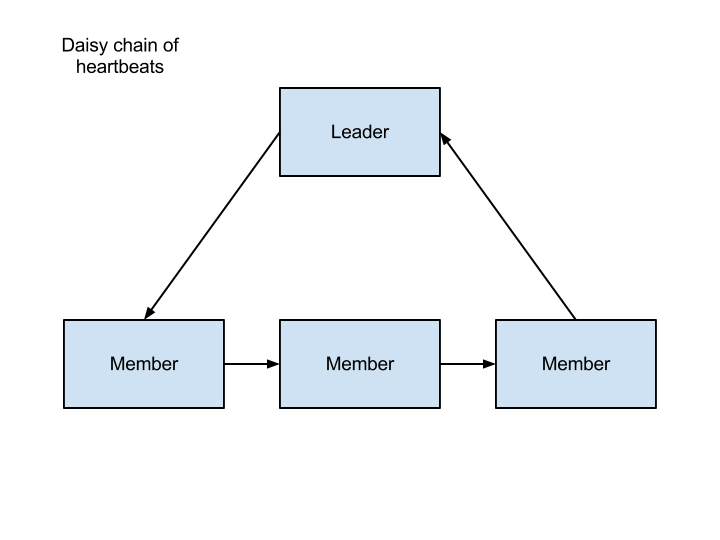
\includegraphics[width=\linewidth]{figures/daisy-chain}
\end{figure}

%\subsubsection{Multi-component nodes}

%Each node maintains a watch list of nodes that it has to monitor health for. The watch list is generated by iterating through all groups and one node from each group that it has to monitor. The watch list is a set, so there will be no duplicate entries, every entry is unique in the watch list.

\paragraph{Message complexity}

Every heartbeat takes one message to send from one to another. As of current,
      we assume every heartbeat is sent using unicast, and there is no ACK for
      heartbeat messages. The message complexity for standard one-hop star
      network takes about
      O(2n-2) messages since the leader sends n-1 to every member and every
      member would also has to send a message back to leader, that comes to
      double of the single traversal from leader to other members.

The message complexity for the daisy loop takes about O(n) messages for a group, because every member only sends one heartbeat to one other member at a time including the leader.

\subsection{Failure recovery}

% mention the needs for at least one substitude, and how the candidate is
% selected

When a node failed, it is guaranteed that at least one node will detect
this. However, the chain is broken, and it would be impossible for the
membership agent in the node to decide what the subsequent actions could be.
They are not designed to do such things.
There need to have another agent to decide based on local information the
actions to take to resolve this issue.

\subsubsection{Link table entry protocol}

% What is link table

When the application is deployed, every operating node contains at least one
object that represents one component in the application. To connect the objects
just like what it did in the application as shown in FBP needs a table to store
the information of the links. Link table is broken down into two layers, where
the top layer gives the information between two components, and the bottom
layer gives a list of nodes that are part of the same group that could provide
the service for operating the application. By breaking into two layers gives
us immense flexibility to handle many different kinds of graph that the FBP could
produce.

% Why a protocol for link table

As illustrated in~\ref{link-table-switch}, the premise of a link between
components rely on both end's agreement. If either one of them disagree, then
the link is not valid.

When a leader of a component failed, the elected new leader will have to update
everyone’s
link table so they all are in consensus of who is currently the representative
for this component. The result of the protocol affects the lower layer of the
link table, so all nodes in the network affiliated with a particular component
could be assure that they are not sending messages to nodes that doesn't exist 
or listening for messages from nodes that are not in charge of sending the
sensor values.

\begin{figure}[h!]
\label{link-table-switch}
\caption{Link table switching}
\centering
    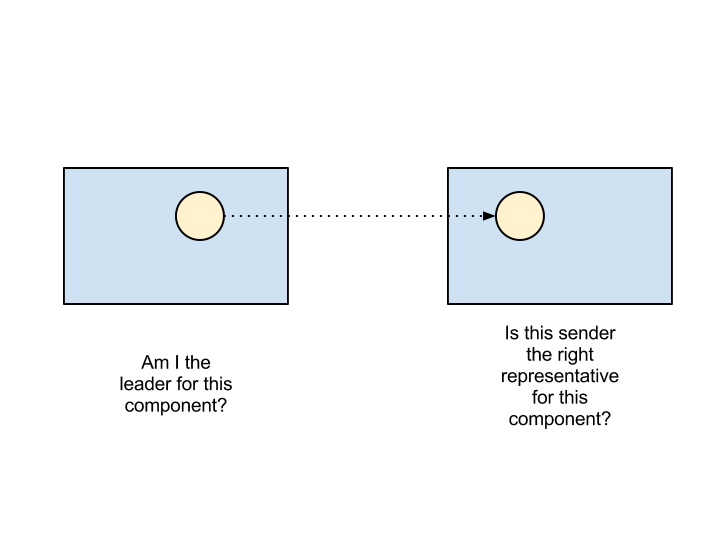
\includegraphics[width=\linewidth]{figures/link-table-switch}
\end{figure}


\subsubsection{Controller agent}

We have described a part of the system that does membership, fault detection.
However with only those parts the system, they do not form a fault tolerant
system. Without a controller making a right decision at the right time,
to synchronize group states, groups will not have consensus and will not be
able to proceed as a whole~\ref{}. Controller’s responsibilities range from
responding to
failure events, synchronizing states to group members and connected nodes to 
ensure the application could still operate.

Reactions and actions tables are set up during deployment. Controller will be
mainly handling events and handle according to the rules defined in the
tables.

\paragraph{Member ranking}

Most other work on failure recovery relies on leader election to elect a new
leader when the old leader failed which is followed by a group multicast to
ensure group state is synchronized to all members.

However, leader election is not necessary if a full member ranking could be
determined. Member ranking serves as a lookup table to successor to any node if it
happens to fail, also used to recover heartbeat network.

%TODO: expend this and explain a bit more with figure and examples

\paragraph{Responding to failure}

~\ref{} describes the dynamics between agents when a failure has been detected.

When a member detected a failure from other member, the membership agent on the
member node will notify local controller agent of this event. 

By default, controller agent will notify the leader of the group if it is not,
the leader’s controller agent will initiate synchronization protocol to
synchronize members’ membership list.

If the leader failed, the controller agent of the monitoring node will initiate
the leader election protocol and become a new leader itself.


\paragraph{Leader election}

% Explain why we need leader election
When there is no clear ranking among members, a leader election could provide a mechanism for determine the successor of a failed node.

% But explain about how member ranking could be used to eliminate leader election

% Then explain that heartbeat network is used as an indication of ranking
% between members



% Need a new figure for leader election with member ranking
%\begin{figure}[h!]
%\caption{Leader election diagram}
%\centering
    %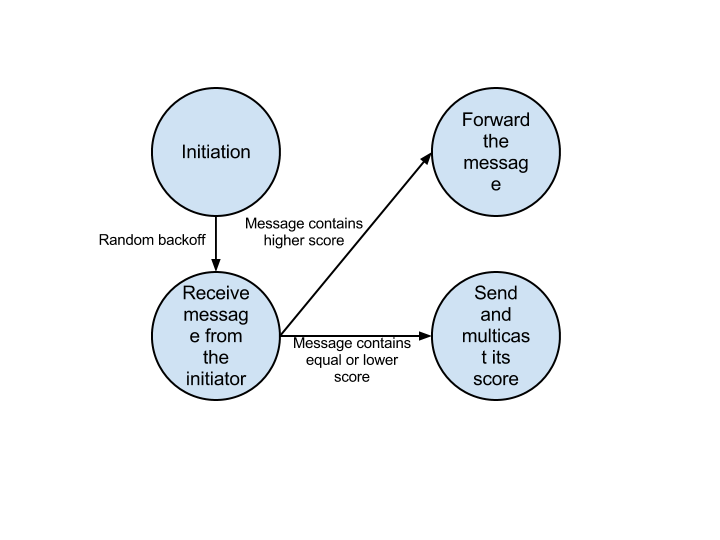
\includegraphics[width=\linewidth]{figures/leader-election-1}
%\end{figure}

\paragraph{Recover from failure}

% confirm and update local membership table


% synchronize membership table in group

\emph{Membership synchronization}

Some actions will be syncing membership list across all members for a particular group. This protocol is triggered either by the reaction table above or by explicit request from other agents, such as the Membership agent. Controller agent will access the current membership table and instruct Synchronization agent to start the membership list synchronization.

% synchronize link table in group and connected nodes

\emph{Link table synchronization}

Once the fault has been confirmed and has shunned the faulty node from the network, GMS coordinator will be responsible for propagating this event to other groups in the system that has subscribe to this event.

Let's say that a group has a simple one hop star topology, so all nodes will transmit its data to the group leader, when the group leader has been reported to be partitioned away from the network or failed, then what will happen is that each group member will elect a new leader by some heuristics, since it has the link table for the previous group leader, it will know which node it is suppose to link to outside the group upstream, and change its local link table accordingly, the new leader will determine the new linking table of its members by consulting the group policy, send a multicast to the group to route all their data to the new leader. The upstream node should either be inside a group managed by the GMS, or a Master assigned gateway, it should also receive this update according to the group policy which GMS will also inform them of.

Essentially, GMS is global in the network and will have full knowledge of the group policy for all groups in the application, and it can follow the group policy to propagation fault events to the appropriate groups.


\subsubsection{False positive fault detection}

It appears to be possible to have false positive fault detection when a node is not dead but actually got partitioned away from the network for a short period of time. If it is the leader that got partitioned away for too long, several members will be detecting this failure and they might all initiate a leader election. Since they all know of this situation, every node detecting a failure will wait for a random amount of time before sending the message. If a leader election message has been received, it will terminate its current action and continue to the second phase of the leader election process.

However, it is possible that leader is not actually dead, and it is also monitoring the members. The leader might conclude that the members are all gone and will also generate a failure event (since there is no one to synchronize to). This is a split brain problem because the remaining members will elect a new leader and proceed in synchronizing the link table in neighbor nodes, but the old leader is still operating and sending data between the neighbor nodes, this will create a conflict both in the group and cause a confusion among the outsiders.

Assuming both partitions can talk to the neighbor nodes with objects connected to their objects, there is no way for the partitions to detect the problem within themselves but only the outsiders.

The outsiders, whose objects are connected to the group, will be the fault detector and will notify both leaders of their existence along with their scoring. The leader with less scoring will give up their leadership, and try to merge with the other partition if possible. If it is still not possible after a timeout, it will try to notify the Master of this situation.

\emph{Daisy chaining}

Since it is also possible that heartbeat is in daisy chain that the any node only monitors one node at a time, and no two nodes monitor the same node. When that happens it is still possible that leader could partition away from the system and appear again later in time. Since the new leader is the one monitoring the old leader, when the old leader resume and start sending heartbeat, the new leader could be sending a reconfiguration message to Master, or if it is not severe enough to do a full reconfiguration, it could resign by sending the old leader a resign message to inform the leader to reconfigure its connected objects about this change of leadership, and it will resume to become a normal member again.

The message complexity for the operation of resignation should be O(2+2H(m)) where H is a function that returns the number of nodes hosting connected objects m.



\subsubsection{Misc. need review}

% TODO:Should I remove this?
\paragraph{Reaction table}

Similar to a routing table, Controller agent will also have a table to look up which actions it could take given a certain type of failure event.

\begin{table}[h!]
\begin{center}
\begin{tabular}{llll}
Source & Detector & Event & Action id \\ 
\hline
“all members” & “any member” & no heartbeat & 0 \\ 
“all members” & “any leader” & no heartbeat & 0 \\
“leader” & “any member” & no heartbeat & 4 \\
\end{tabular}
\end{center}
\caption{An example of reaction table}
\end{table}


% TODO:Should I remove this?
\paragraph{Action table}

This table list all actions that a controller could do. This table follow similar style described in the work of ADAE with rules that provides graceful degradation for most actions.

\begin{table}[h!]
\begin{center}
\begin{tabular}{llllllll}
Id & Profile type & Next & Secondary & Doer & Receiver & Function & Expected
results \\
\hline
0 & standard & 3 & 1 & “leader” & “all members” & “member list synchronization” & “member list synced” \\
1 & secondary &  &  & “leader” & “operating members” & “member list synchronization” & “member list synced” \\
2 & standard &  &  & “any member” & “leader” & “send” & “relay event” \\
3 & standard &  &  & “leader” & “all members and connected nodes” & “link table synchronization” & “link table updated” \\
4 & standard &  &  & “operating members” & “operating members” & “leader election” & “a new leader elected” \\
\end{tabular}
\end{center}
\caption{An example of action table}
\end{table}

When a standard action failed, the secondary action will be triggered, for example, if action 0 failed, action 1 will take over since it is a secondary of action 0. When action 0 finish execution, action 3 will follow it immediately since it is a next of action 0.

% TODO:Should I remove this?
\paragraph{Event queue}

Controller will be bombarded by lots of events coming from multiple sources in a short period of time, to ensure all events are stored in chronological or importance order, a event queue is used. Any event that other agents send to notify controller will be stored in this queue.

\begin{table}[h!]
\begin{center}
\begin{tabular}{ll}
Event name & Priority \\
\hline
“No heartbeat” & 0 \\
“Event queue synchronization” & 1 \\
\end{tabular}
\end{center}
\caption{Event queue}
\end{table}



% TODO:Should I remove this?
\emph{Event queue synchronization}

It is very likely that if nodes failed, the events carried on the nodes will never see the light of day in other nodes, and will never be handled. To prevent missing events, controller will have to synchronize event queue among members.

\emph{Preemptive event queue}

Some events have higher priority, and those events should come in in sparse intervals. Event queue synchronization is an important event that any controller should preempted before other unhandled events.

